\begin{figure}[!h]
\centering
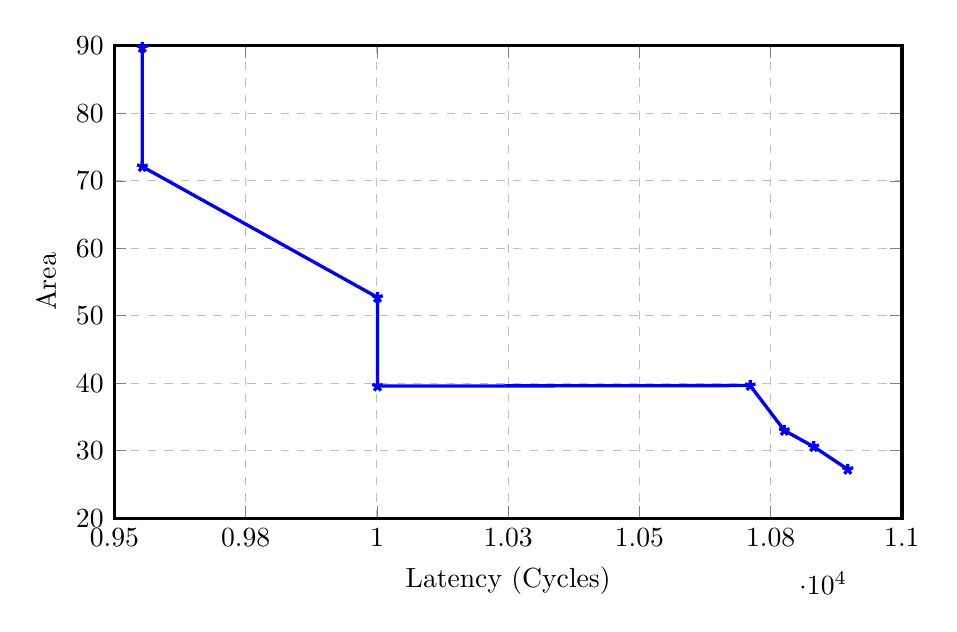
\begin{tikzpicture}
\begin{axis}[
scale only axis,
height=6cm,
width=10cm,
    xlabel={Latency (Cycles)},
    ylabel={Area},
    xmin=9500, xmax=11000,
    ymin=20, ymax=90,
    xtick={9500,9750,10000,10250,10500,10750,11000},
    ytick={20,30,40,50,60,70,80,90},
    legend pos=north east,
    ymajorgrids=true,
    xmajorgrids=true,
    grid style=dashed,
    very thick
]
\addplot[
    color=blue,
    mark=star,
   % smooth
    ]
    coordinates {
    (9553,89.745)(9553,72.098)(10001,52.720)(10001,39.579)(10711,39.658)(10776,33.004)(10832,30.595)(10897,27.2395)
    };
\end{axis}
\end{tikzpicture}
\caption{Area Vs. Latency Curve for 128-Point FFT Implementation}
\label{plot_128fft}
\end{figure}